\documentclass[12pt]{article}

\usepackage{graphicx}
\usepackage{epstopdf}


\usepackage[spanish]{babel} % silabea palabras castellanas <- Puedo poner comentarios para explicar de que va este comando en la misma línea
\selectlanguage{spanish} 

%Encoding
\usepackage[utf8]{inputenc} % Acepta caracteres en castellano
\usepackage[T1]{fontenc} % Encoding de salida al pdf

%Triunfó el mal
\usepackage[normalem]{ulem}
\useunder{\uline}{\ul}{}
\providecommand{\e}[1]{\ensuremath{\times 10^{#1}}}
\usepackage{quotmark} %Uso consistente con la RAE de comillas
\usepackage{listings} % Comandos de la terminal

\usepackage{textcomp}
\usepackage{gensymb}


%Hipertexto
\usepackage[colorlinks=true,urlcolor=blue,linkcolor=blue]{hyperref} % navega por el doc: hipertexto y links

%Aquello de las urls
\usepackage{url} 

%simbolos matemáticos
\usepackage{amsmath}
\usepackage{amsfonts}
\usepackage{amssymb}
\usepackage{physics} %Best pack

% permite insertar gráficos, imágenes y figuras, en pdf o en eps
\usepackage{graphicx}
\usepackage{epstopdf}
\usepackage{multirow}
\usepackage{float}
\usepackage[export]{adjustbox}
% geometría del documento, encabezados y pies de páginas, márgenes
\usepackage{geometry}
\usepackage{comment}

%\usepackage[english]{babel}
%\usepackage[latin5]{inputenc}
% \usepackage{hyperref}
%\newdate{date}{10}{05}{2013}
%\date{\displaydate{date}}
\begin{document}




\title{Cúmulos Abiertos \\ Correcciones CCD 1 IRAF}

\author{
\textbf{Javier Alejandro Acevedo Barroso\thanks{e-mail: \texttt{ja.acevedo12@uniandes.edu.co}}}\\
\textit{Universidad de los Andes, Bogotá, Colombia}\\
 }% Hasta aquí llega el bloque "author" (son dos autores por informe, orden alfabético)

\date{\today}
%\date{Versión $\alpha \beta$ fecha del documento}
\maketitle %Genera el título del documento


\normalsize
\newpage





\section{Image Reduction and Analysis Facility}
Image Reduction and Analysis Facility (IRAF) es un software de reducción y análisis de imágenes mantenido por la \tqt{National Optical Astronomy Observatories} (NOAO) en Estados Unidos. El proyecto IRAF nace en 1981 en el Observatorio Nacional Kitt Peak, en donde de 1982 a 1984 se escribió la primera versión del software y su lenguaje de script para el usuario \tqt{Command Language} (CL). En 1984 empezó su uso científico en el \tqt{Space Telescope Science Institute} impulsando la implementación del software en diferentes arquitecturas de máquinas de la época, en particular, se implementó para la arquitectura UNIX en 1986. Para principios de la siguiente década IRAF es el estandar científico de procesamiento de imagen en Estados Unidos y observatorios asociados\cite{IRAFinThe80}. \\
Así mismo, durante esa década el softwafe se adaptó a las innovaciones tecnológicas, tales como: la programación orientada a objetos, que surge del refinamiento de las prácticas de programación durante los ochenta; las redes de computadores, en particular la recien nacida World Wide Web; las interfaces de usuario, que en el caso de IRAF evolucionó a XGterm y DS9; y los lenguajes de programación de alto nivel, que en ese momento eran C, C++ y Fortran\cite{IRAFinThe90}.\\
Para el nuevo milenio IRAF era el estándar mundial en reducción y análisis de imagen astronómicas, por encima de proyectos similares como \tqt{Starlink Project} que fue también un softwafe de reducción y procesamiento de datos pero escrito por la comunidad astronómica de Reino Unido.\\
IRAF está organizado en \tqt{paquetes} que contienen rutinas específicas denomidadas \tqt{tareas}. Cada paquete agrupa tareas relacionadas de acuerdo a su uso. Por ejemplo, hay paquetes que traen todo lo relacionado a la descompresión y carga de imágenes, o paquetes dedicados a ciertos tipos de análisis como astrometría o fotometría.



\section{SAOImageDS9}
SAOImageDS9 (comunmente llamado DS9) es un software de visualización y creación de imágenes a partir de datos. Las principales particularidad de DS9 son: Dado lo temprano de su desarrollo, sus algoritmos fueron un fuerte avance no solo para la astronomía, sino también para la visualización computacional en sí; su capacidad de procesar archivos de formato .fits, que es el formato más utilizado en astronomía; y la fácil comunicación con herramientas de análisis externas, como IRAF, permitiendo realizar el procesamiento de los datos en un ordenador diferente al que se usa para la visualización.\\
La historia de DS9 empieza en 1990 cuando Mike Van Hilst escribe SAOImage en el \tqt{Smithsonian Astrophysical Observatory} (SAO). El software, siendo uno de los primeros en su tipo, representó tecnicas innovadoras en la visualización de datos, al punto de que hoy muchos programas de visualización de datos implementan algoritmos originalmente de SAOImage. El éxito inicial de SAOImage llevó al desarrollo durante los noventa de \tqt{SAOImage, The Next Generation}, que extendió la funcionalidad de SAOImage a nuevos entornos gráficos (nótese que fue en esta década que se desarrollaron los GUI como los entendemos hoy). Por último, finales de los noventa, se desarrolló el sucesor a \tqt{SAOImage, The Next Generation}, que llamaron \tqt{SAOImageDS9} para continuar con un esquema de nombres relacionado a Star Trek (The Next Generation y Deep Space 9 son los títulos de diferentes series que toman lugar en el universo de Star Trek). La primera versión de DS9 fue lanzada al público en 1999, y,gracias al financiamiento de NASA y el \tqt{Chandra X-Ray Science Center} entonces ha recibido soporte continuo de parte de SAO. La versión actual de DS9 es la 7.6 estable y la 8 en beta.\cite{ds9}





\section{Reporte de la instalación de IRAF}
Dada la época en donde se escribió la primera versión del software, la interfaz de usuario de IRAF es bastante robusta. Si bien, se ha recopilado paquetes binarios para instalar IRAF usando un instalador automático, la necesidad de usar librerías no incluidas y software adicional como \tqt{ximtools}, así como los diferentes niveles de permisos que requiere IRAF durante su instalación, dan lugar a un zoológico de errores posibles.\\
Por lo anterior, la instalación de IRAF tomó numerosos intentos. El software se instaló en un computador de mesa y un portátil comercial, ambos con instalaciones funcionales de Ubuntu 18.04. Los primeros intentos de instalación fallaron por errores a la hora de elegir los paquetes binarios a descargar, pues estos deben coincidir no solo con el sistema operativo (Linux) sino también con la arquitectura del procesador. Las siguientes instalaciones sufrieron de problemas a la hora de obtener las librerías de Linux que requiere IRAF pues estas cambiaron ligeramente de nombre. Tras varios intentos se logró tener una instalación exitosa en el computador de mesa, sin embargo, en el computador portatil hay errores adicionales, pues nunca se puede ejecutar correctamente el comando \tqt{ecl}. Finalmente se optó por usar el computador de mesa para el trabajo en IRAF y el portatil únicamente para tomar nota de los comandos en clase.\\
La instalación exitosa se realizó utilizando un tutorial de la universidad de Ohio para linux de 64 bits\cite{OhioTutorial}. Dado el cambio en el nombre de los paquetes, esta es la versión correcta del comando a usar:

\begin{lstlisting}[language=bash]
sudo apt install tcsh libxss1 lib32z1 lib32ncurses5 
libxmu-dev libbz2-1.0:i386 
\end{lstlisting}

Para verificar el éxito de una instalación se creo una instancia de XGterm y desde ahí se ejecuta el IRAF. Si se obtiene la pantalla de bienvenida de IRAF sin error alguno, entonces se tuvo una instalación exitosa ver figura \ref{im0}.

\begin{figure}[H]
  \centering
   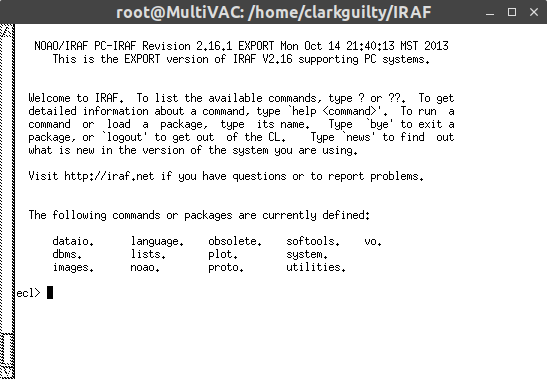
\includegraphics[scale= 0.65]{im0.png}
  \caption{Sesión de XGterm con la pantalla de bienvenida de IRAF, muestra de una instalación exitosa.}
  \label{im0}
\end{figure}



\section{Ejercicios}
El ejercicio consiste en seguir el tutorial de IRAF \tqt{intro.txt}. En este tutorial se presentan algunas tareas y paquetes básicos del programa, para luego hacer un ejercicio de alinear dos imágenes ligeramente corridas entre sí, y promediarlas después. A continuación se presentarán los comandos que considero prudente registrar para futuras referencias y algunos de sus resultados:\\
Para descomprimir imágenes se debe primero cargar el paquete \tqt{rfits}, esto se hace utilizando el comando \tqt{unlearn}. Una vez cargado el paquete, se procede a descomprimir las imágenes.	

\begin{figure}[H]
  \centering
   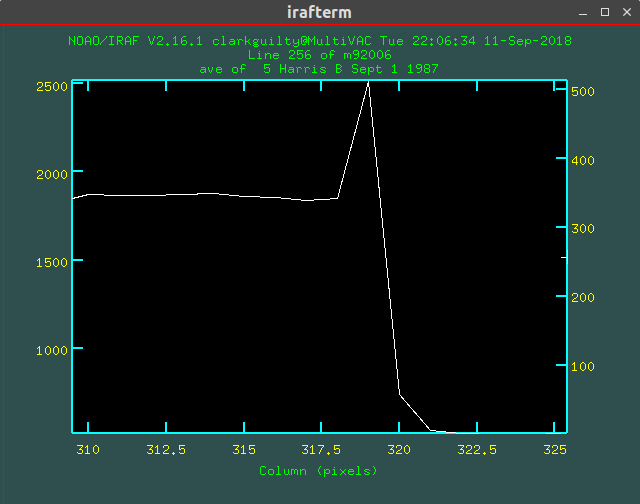
\includegraphics[scale= 0.65]{im01.png}
  \caption{Carga de rfits y sucesiva descompresión de imágenes. se listó los archivos del directorio para confirmar que sí se generaran los .fits. }
  \label{im01}
\end{figure}

Para visualizar los parámetros ocultos de una tarea se usa el comando \tqt{lpar}, para modificarlos se usa \tqt{epar} (ver imagen \ref{im02}. Es importante recordar que cuando se edita texto desde la terminal, este se debe guarda usando \tqt{:qt}. 

\begin{figure}[H]
  \centering
   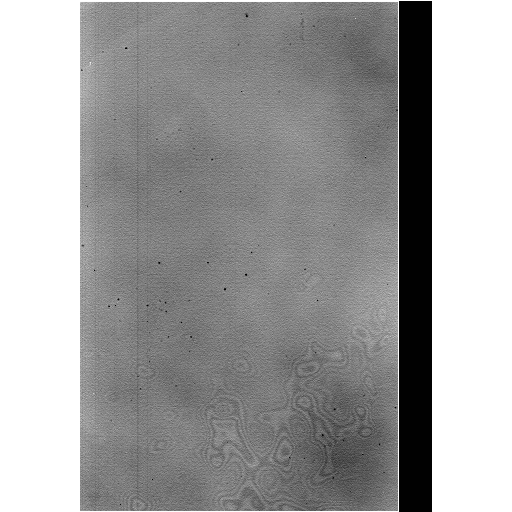
\includegraphics[scale= 0.65]{im02.png}
  \caption{Modificando los parámetros ocultos de imhead usando epar.}
  \label{im02}
\end{figure}

Procediendo ahora al ejercicio en sí, este empieza explicando el uso de \tqt{DS9}. Primero se debe ejecutar en una terminal de Linux (nótese que ya se tenía abierta la sesión de xgterm con IRAF):

\begin{lstlisting}[language=bash]
ds9
\end{lstlisting}

Para mostrar una imagen, basta con usar el comando \tqt{display}. Como DS9 tiene cuatro recuadros para imágenes, al usar la tarea \tqt{display} (ver imagen \ref{im03}) se debe señalar que recuadro de DS9 se va a usar. Se abrió DS9 y se cargó las dos imágenes
\begin{figure}[H]
  \centering
   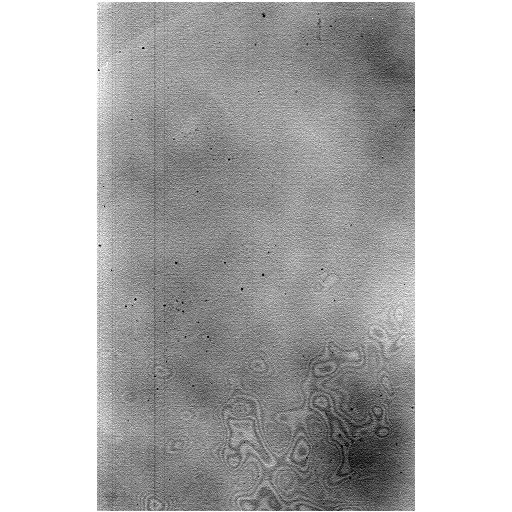
\includegraphics[scale= 0.65]{im03.png}
  \caption{Cargando las imágenes a diferentes frames de DS9 desde la sesión de IRAF. }
  \label{im03}
\end{figure}




Ahora, para alinear las imágenes, se ubicarán más de diéz estrellas en ambas imágenes y con ello se calcula el corrimiento entre ellas. Sin embargo, no todos los puntos son necesariamente estrellas. Para verificar si un punto es una estrella se debe estudiar el perfil radial, esto se hace con la tarea \tqt{imexamine}. Tras ejecutar la tarea en la sesión de IRAF, se vuelve a DS9, en donde el cursero ha cambiado a modo interactivo. Para cada punto candidato a estrella, se ubica el cursor en él y se presiona la tecla \tqt{r}, si todo se hizo correctamente (y no se está usando la versión 7.2 de DS9 pues tiene un bug en el cálculo de las coordenadas del cursor) se debe obtener una nueva ventana con la gráfica del perfil radial (ver imagen \ref{im05}). 


\begin{figure}[H]
  \centering
   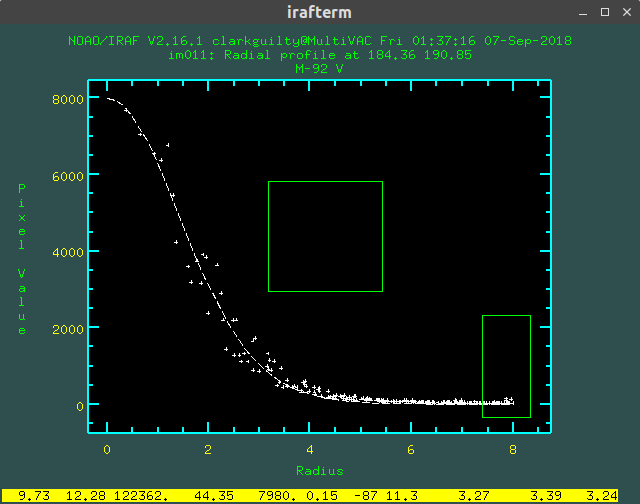
\includegraphics[scale= 0.6]{im05.png}
  \caption{Perfil radial de un buen candidato a estrella. Nótece lo ceñido que están los puntos a la línea de tendencia, esto es una cuantificación visual de que tanto se ajusta el perfil radial del punto al de una estrella.}
  \label{im05}
\end{figure}

La gráfica generada muestra el valor del pixel contra distancia al centro del punto, y lo contrasta con una línea de tendencia. Si la fuente es una estrella, se espera que los puntos estén cerca a la línea de tendencia pues son emitidos por una fuente coherente y no son ruido aleatorio. La figura \ref{im05} es un ejemplo de un buen candidato a estrella. Un mal candidato a estrella tiene mucha mayor dispersión. 



\begin{figure}[H]
  \centering
   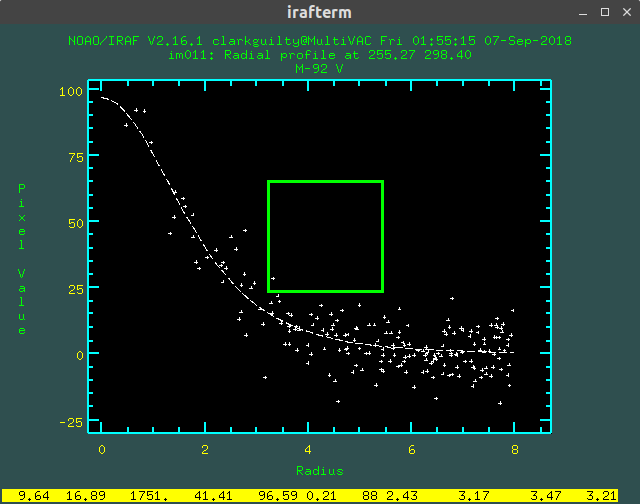
\includegraphics[scale= 0.6]{im06.png}
  \caption{Perfil radial de un mal candidato a estrella. Se observa alta dispersión respecto a la línea de tendencia. y que el máximo del valor del pixel no es muy grande, incluso se observan valores del pixel negativos}
  \label{im06}
\end{figure}

Una vez seleccionados los candidatos razonables, y diferenciando con un circulo verde (ver figura \ref{im07}), se debe tomar la posición de cada uno y contrastarla con la posición de la misma estrella en la otra imagen. Al promediar la diferencia se obtiene un vector de corrimiento ($\vec{d}$). Dejando fija la imagen \tqt{im010}, las nuevas coordenadas de \tqt{im011} estarán dadas por:
\begin{equation}
\vec{x'}= \vec{x} + \vec{d}
\end{equation}
Usando Python para promediar se obtiene un vector $\vec{d} = -0.54\vu{x} -1.64\vu{y}$\\
Por último, tanto el código utilizado, como los datos de las estrellas tomadas se  encuentran en el repositorio de github \url{https://github.com/ClarkGuilty/2018/tree/master/Astronomia/tareaIraf1}

\begin{figure}[H]
  \centering
   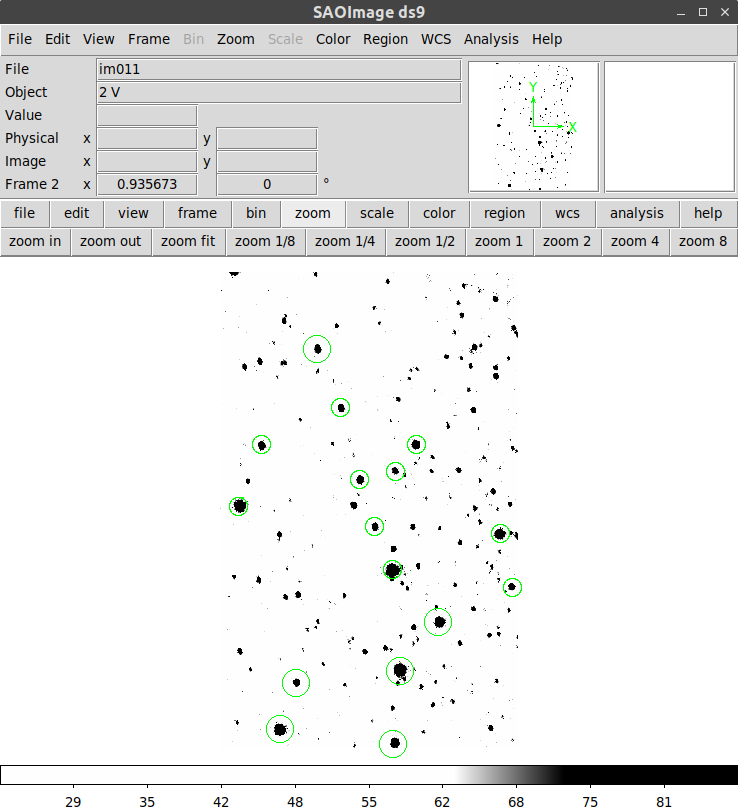
\includegraphics[scale= 0.65]{im07.png}
  \caption{Candidatos a estrella seleccionados por su perfil radial. No se pudo seleccionar ningún buen candidato de la región superior derecha.}
  \label{im07}
\end{figure}



\bibliography{bibTes}{}
\bibliographystyle{unsrt}














\end{document}








\section{Cronograma}

\begin{table}[htb]
	\begin{tabular}{|c|cccccccccccccccc| }
	\hline
	Tareas $\backslash$ Semanas & 1 & 2 & 3 & 4 & 5 & 6 & 7 & 8 & 9 & 10 & 11 & 12 & 13 & 14 & 15 & 16  \\
	\hline
	1 & X & X & X  &   &   &   &   &  &  &   &   &   &   &   &   &   \\
	2 &   &  & X & X & X &  &  &   &   &  &  &  &   &  &  &   \\
	3 &   &   &   &  & X  & X  & X  & X &   &   &   &  &   &   &  &   \\
	4 &  &  &  &  &  &  &  & X & X & X & X &   &   &   &   &   \\
    5 &  &  &  &  &  &  & X & X &  &  &  &   &   &   &   &   \\
	6 &   &   &   &   &  &   &  X & X  &  &   &  X & X &  X & X  & X &   \\
	\hline
	\end{tabular}
\end{table}
\vspace{1mm}
 